\documentclass[11pt]{article}

\usepackage{amsfonts}
%\usepackage{geometry}
\usepackage[paper=a4paper, 
            left=20.0mm, right=20.0mm, 
            top=25.0mm, bottom=25.0mm]{geometry}
\pagestyle{empty}
\usepackage{graphicx}
\usepackage{fancyhdr, lastpage, bbding, pmboxdraw}
\usepackage[usenames,dvipsnames]{color}
\definecolor{darkblue}{rgb}{0,0,.6}
\definecolor{darkred}{rgb}{.7,0,0}
\definecolor{darkgreen}{rgb}{0,.6,0}
\definecolor{red}{rgb}{.98,0,0}
\usepackage[colorlinks,pagebackref,pdfusetitle,urlcolor=darkblue,citecolor=darkblue,linkcolor=darkred,bookmarksnumbered,plainpages=false]{hyperref}
\renewcommand{\thefootnote}{\fnsymbol{footnote}}

\pagestyle{fancyplain}
\fancyhf{}
\lhead{ \fancyplain{}{Course Name} }
%\chead{ \fancyplain{}{} }
\rhead{ \fancyplain{}{\today} }
%\rfoot{\fancyplain{}{page \thepage\ of \pageref{LastPage}}}
\fancyfoot[RO, LE] {Page \thepage\ of \textcolor{black}{\pageref{LastPage}} }
\thispagestyle{plain}

%%%%%%%%%%%% LISTING %%%
\usepackage{listings}
\usepackage{caption}
\usepackage{subcaption}
\DeclareCaptionFont{white}{\color{white}}
\DeclareCaptionFormat{listing}{\colorbox{gray}{\parbox{\textwidth}{#1#2#3}}}
\captionsetup[lstlisting]{format=listing,labelfont=white,textfont=white}
\usepackage{verbatim} % used to display code
\usepackage{fancyvrb}
\usepackage{acronym}
\usepackage{amsthm, amsmath}
\usepackage{tikz}
    \usetikzlibrary{calc, arrows, arrows.meta, positioning}
\usepackage{amssymb,amsmath,stackengine}
\stackMath
\usepackage{ifthen}

\VerbatimFootnotes % Required, otherwise verbatim does not work in footnotes!

\definecolor{OliveGreen}{cmyk}{0.64,0,0.95,0.40}
\definecolor{CadetBlue}{cmyk}{0.62,0.57,0.23,0}
\definecolor{lightlightgray}{gray}{0.93}

\lstset{
	%language=bash,                          % Code langugage
	basicstyle=\ttfamily,                   % Code font, Examples: \footnotesize, \ttfamily
	keywordstyle=\color{OliveGreen},        % Keywords font ('*' = uppercase)
	commentstyle=\color{gray},              % Comments font
	numbers=left,                           % Line nums position
	numberstyle=\tiny,                      % Line-numbers fonts
	stepnumber=1,                           % Step between two line-numbers
	numbersep=5pt,                          % How far are line-numbers from code
	backgroundcolor=\color{lightlightgray}, % Choose background color
	frame=none,                             % A frame around the code
	tabsize=2,                              % Default tab size
	captionpos=t,                           % Caption-position = bottom
	breaklines=true,                        % Automatic line breaking?
	breakatwhitespace=false,                % Automatic breaks only at whitespace?
	showspaces=false,                       % Dont make spaces visible
	showtabs=false,                         % Dont make tabls visible
	columns=flexible,                       % Column format
	morekeywords={__global__, __device__},  % CUDA specific keywords
}

\newcommand{\question}[1]{\section*{\normalsize #1}}
% \newcommand{\mat}[1]{\begin{bmatrix}#1\end{bmatrix}}
% \newcommand{\extraspace}[]{
%     \begin{center}
%         \textbf{Use this page for extra space.}
%     \end{center}
% }


\DeclareMathOperator*{\argmax}{arg\,max}
\DeclareMathOperator*{\argmin}{arg\,min}
%\DeclareMathOperator*{\vec}[1]{\textbf{#1}}

\newcommand{\squig}{{\scriptstyle\sim\mkern-3.9mu}}
\newcommand{\lsquigend}{{\scriptstyle\lhd\mkern-3mu}}
\newcommand{\rsquigend}{{\scriptstyle\rule{.1ex}{0ex}\rhd}}
\newcounter{sqindex}
\newcommand\squigs[1]{%
  \setcounter{sqindex}{0}%
  \whiledo {\value{sqindex}< #1}{\addtocounter{sqindex}{1}\squig}%
}
\newcommand\rsquigarrow[2]{%
  \mathbin{\stackon[2pt]{\squigs{#2}\rsquigend}{\scriptscriptstyle\text{#1\,}}}%
}
\newcommand\lsquigarrow[2]{%
  \mathbin{\stackon[2pt]{\lsquigend\squigs{#2}}{\scriptscriptstyle\text{\,#1}}}%
}


\begin{document}
\begin{center}
    {\Large \textsc{Written Assignment 2}}
\end{center}
\begin{center}
    Due: Friday 02/16/2024 @ 11:59pm EST
\end{center}

\section*{\textbf{Disclaimer}}
I encourage you to work together, I am a firm believer that we are at our best (and learn better) when we communicate with our peers. Perspective is incredibly important when it comes to solving problems, and sometimes it takes talking to other humans (or rubber ducks in the case of programmers) to gain a perspective we normally would not be able to achieve on our own. The only thing I ask is that you report who you work with: this is \textbf{not} to punish anyone, but instead will help me figure out what topics I need to spend extra time on/who to help. When you turn in your solution (please use some form of typesetting: do \textbf{NOT} turn in handwritten solutions), please note who you worked with.\newline

\noindent Remember that if you have a partner, you and your partner should submit only \textbf{one} submission on gradescope.



\question{Question 1: Gradient Descent (25 points)}
Given two vectors $\hat{\vec{y}}^{(t)}\in \mathbb{R}^{n}$ and $\vec{y}\in \mathbb{R}^{n}$, we can measure the distance between them using the following objective function:
$$L\Big(\hat{\vec{y}}^{(t)}, \vec{y}\Big) = \frac{1}{2}\sum\limits_{i=1}^n \Big(\hat{y}_i^{(t)} - y_i\Big)^2$$

\noindent Assume that $\hat{\vec{y}}^{(t)}$ is the output of an Agent at time $t$ and that we wish to improve using gradient descent by minimizing the distance between $\hat{\vec{y}}^{(t)}$ and $\vec{y}$. Calculate the gradient $\nabla_{\hat{\vec{y}}^{(t)}} L$ that we would need to implement in our code to execute the gradient descent algorithm.

\bigskip
We can separate the summation into each dimension. For example, for $i=7$, we have

\[\frac{1}{2} \times 2 \times \Big(\hat{y}_7^{(t)} - y_7\Big)^1 = \hat{y}_7^{(t)} - y_7\]

Thus, our gradient is

\[\left( \hat{y}_1^{(t)} - y_1,\, \hat{y}_2^{(t)} - y_2,\, \hat{y}_3^{(t)} - y_3,\, \dots ,\, \hat{y}_n^{(t)} - y_n\right)\]

\newpage

\question{Question 2: Hill Climbing Optimality (25 points)}
Consider the following world (shown from an arial top-down view):

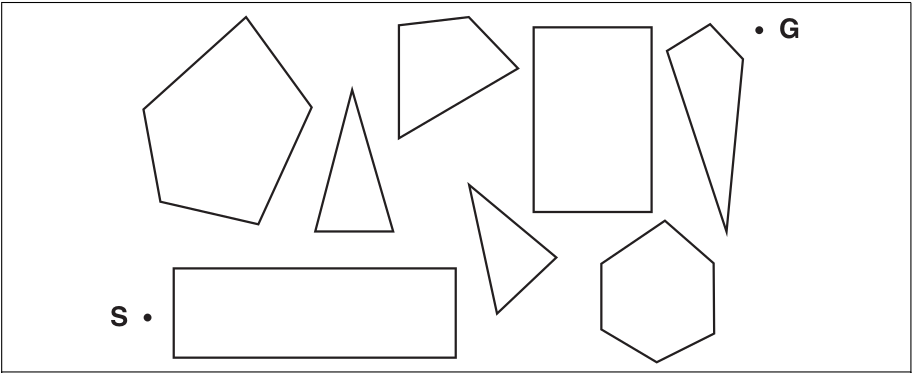
\includegraphics[width=0.8\linewidth]{./imgs/polygon_hill_climbing_map.png}

\begin{enumerate}
    \item[a)] Consider discretizing this world (i.e. laying a grid down on top of the world so we see a discrete coordinate system). Assume that the discretization is a fine as required (but not continuous) to preserve the geometry of the shapes present in the world. A \textit{convex} shape is a shape where if we were to draw a line between any two points of the shape, the line would entirely be contained \textit{within} the shape. Given a world that contains convex \textit{obstacles}, is it possible for a vanilla hill climbing agent to get stuck?

    \item[b)] What if we could prove that the \textbf{objective surface} was convex. Would it be possible for a vanilla hill climbing agent to get stuck?
\end{enumerate}

\bigskip

\begin{enumerate}
	\item[a)] \textbf{Yes}, because we could be faced with an edge which is perpendicular to the direct line of travel to $G$. In this case, the best we can do is turn 90° to the left or right, neither of which will increase our objective function (they will actually decrease it because the hypotenuese is the longest side of a right triangle; one leg is the direct line from $S$ to $G$ and the other leg is in the direction that we are turning.)
	\item[b)] \textbf{No...} If the objective surface is convex, any local minima are global minima. That is, there is no chance for us to get stuck in a local minima while there is a better state outside of our immediate neighborhood. Even if there were multiple global minima, this would imply that there are several equally desirable states, so the hill climber would find one of them.
	
	% However, if we allow for ``plateaus'' in the objective function, it's possible for a vanilla hill climber to get stuck. We would descend down to the edge of the plateau and then stop, even if the goal was in the middle of the plateau. Really though, we would still be at a global minimum so in the context of the problem we would have reached a goal state.
\end{enumerate}

\newpage


\question{Extra Credit: Gradient Descent and Lipshitz Continuity (50 points)}
Gradient Descent is the continuous version of hill climbing where we use the gradient of the objective function to measure which direction leads uphill (we can then decide whether or not to follow the gradient uphill or downhill). Let us consider going downhill (i.e. we are choosing to \textit{minimize}). The trouble is that gradient descent is a local search algorithm, meanining that it is not guaranteed to:
\begin{itemize}
    \item Converge at all. There may not be any local minima to find.
    \item Arrive at the global minima if one exists.
\end{itemize}

\noindent A function $f$ is \textit{Lipschitz Continuous} with constant $k>0$ if $\forall \vec{x},\vec{y} \hspace{.5cm}||f(\vec{x})-f(\vec{y})||_2\le k||\vec{x}-\vec{y}||_2$. Think of it this way: for every pair of points, $f$ is bounded on how fast it can change by $k$. \href{https://en.wikipedia.org/wiki/Lipschitz_continuity}{Here} is a good gif that visualizes lipschitz continuity.\newline

\noindent If we know that our objective function $f: \mathbb{R}^n \rightarrow \mathbb{R}$ is convex and differentiable, \textit{and} we know that the gradient of $f$ (i.e. $\nabla f$) is Lipschitz continuous with (minimum) constant $c > 0$, prove that \textbf{not only} is gradient descent \textbf{guaranteed} to converge (for specific values of the step size $\eta$), but that it \textbf{will} converge if $\eta \le \frac{2}{c}$.\newline\newline
\noindent Hint: you may find it useful to use a 2nd degree taylor polynomial of $f$ centered around $f(\vec{x})$, which can be expressed as:
$$f(\vec{y}) \le f(\vec{x}) + \nabla f(\vec{x})^T (\vec{y}-\vec{x}) + \frac{1}{2}(\vec{y}-\vec{x})^T\nabla^2 f(\vec{x})(\vec{y}-\vec{x})$$

Local min is global min for convex surfaces, so we don't have any risk of falling into a small valley (not possible to get stuck)


\end{document}

